\documentclass{standalone}
\usepackage{tikz}

\begin{document}
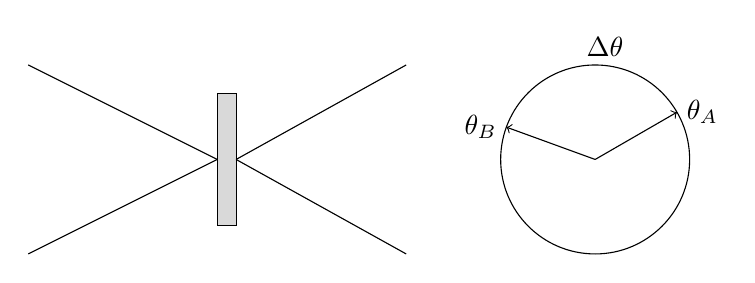
\begin{tikzpicture}[scale=1.2]
  % input lines
  \draw (-2,1) -- (0,0);
  \draw (-2,-1) -- (0,0);
  % beamsplitter
  \draw[fill=gray!30] (0,-0.7) rectangle (0.2,0.7);
  % output lines
  \draw (0.2,0) -- (2,1);
  \draw (0.2,0) -- (2,-1);

  % phase circle
  \begin{scope}[xshift=4cm]
    \draw (0,0) circle(1);
    \draw[->] (0,0) -- (30:1) node[right]{$\theta_A$};
    \draw[->] (0,0) -- (160:1) node[left]{$\theta_B$};
    \node at (85:1.2) {$\Delta\theta$};
  \end{scope}
\end{tikzpicture}
\end{document}